\chapter{Aufbau}
\label{ch:Aufbau}
Dieses Kapitel beschreibt den konkreten Aufbau der Testbench. Wie in Sektion \ref{sec:Architektur und Technologien:Architektur} beschrieben, ist die verwendete Architektur Event-basiert. Abbildung \ref{fig:classDiagram} skizziert eine vereinfachte Form der Testbench in einer UML-Klassendiagramm ähnlichen Form. Aus Übersichtsgründen sind Utility-Klassen, Transfer-Objekte, POJO's\footnote{Plain Old Java Objects: Werden bspw. für die JSON-Deserialisierung benutzt} und die Event-Listener/Event-Publisher der Komponenten nicht Teil des Diagramms. Für jede Komponente, die eine Nachricht in Form eines Events an andere schicken oder von anderen empfangen möchte, existiert ein Listener beziehungsweise ein Publisher. Methoden des Listeners delegieren nach Empfang von Events die erhaltenen Nachrichten (Methodenaufrufe) an ihre nachgeschaltete Komponente. Komponenten die Nachrichten senden wollen, überreichen diese an ihren jeweiligen Publisher, der diese in Form eines Events auf den Event-Bus legt. Näheres ist in Sektion \ref{sec:Aufbau:Events} erklärt. \\
Im Folgenden werden alle wichtigen Systemkomponenten erläutert. Anschließend wird ein Überblick über die verschiedenen Event-Typen gegeben. Danach wir der zeitliche, sich periodisch wiederholende Ablauf eines Intervalls in der Testbench vorgestellt.









\section{Komponenten}
Abbildung \ref{fig:classDiagram} beschreibt den Zusammenhang aller Kern-Komponenten des Auto-Skalierers. Der Event-Bus selbst wird vom Spring-Framework bereitgestellt und ist nicht selbst implementiert. Die \textit{<<use>>} Bezeichnung soll lediglich verdeutlichen, dass die Komponenten Listener und/oder Publisher vorgeschaltet haben, die mit dem Event-Bus interagieren. Aus Gründen der Übersicht existieren keine Assoziations-Pfeile zwischen dem \textit{ApplicationStartUpRunner} und den Komponenten, die er initialisiert. Die Methodennamen lassen aber darauf schließen, mit welcher Komponente noch eine Assoziation existiert.

\subsection{Clock}
\label{sec:aufbau:Clock}
Die \textit{Clock} erfüllt die Aufgabe eines Taktgebers und ist somit das Herz der Testbench. In einer zeit-diskreten Simulation ist es solcher Taktgeber notwendig, da jede Komponenten über den Beginn eines neuen Intervalls informiert werden muss. Dabei gilt: Ein Intervall gilt erst dann als beendet, sobald jede Komponente ihre Aufgaben innerhalb dieses Intervalls erledigt hat. Nach Initialisierung der Komponenten arbeitet die Clock für eine in der Konfiguration definierte Anzahl an Intervallen (Simulationszeit). Dabei wird in jedem Schritt zuerst der Workload, falls notwendig, geändert. Danach versendet die Clock ein Event, dass den Beginn eines neuen Intervalls bekannt gibt. Alle Komponenten werden benachrichtigt und erledigen daraufhin ihre Arbeit, wie Verarbeitung der aktuell anliegenden Workload oder Ausführen von Skalier-Entscheidungen. Abschließend werden \textit{InfrastructureModel} und \textit{QueueModel} durch die Clock aufgefordert ihren aktuellen Zustand zu publizieren. Basierend darauf führen die Komponenten im nächsten Intervall ihre Aufgaben durch. 


\subsection{Infrastructure Model}
Das \textit{InfrastructureModel} bündelt die Haupt-Komponenten der Testbench. Es hat eine Warteschlange für ankommende und wartende Jobs (vgl.\ref{sec:aufbau:QueueModel}), eine Komponente die sich um das Hochfahren der Virtuellen Maschinen kümmert (vgl.\ref{sec:aufbau:BootinQueu}) sowie einen gekapselten Zustand (vgl.\ref{sec:aufbau:State}). \\
Die Information, wie viel Last in welchem Zeitintervall anliegt, wird im \textit{InfrastructureModel} gespeichert und ggf. durch Erhalt einer Workload-Änderung (\textit{changeWorkload()}) geändert. Basierend darauf, ist sie verantwortlich bei Erhalt eines jeden Clock-Ticks (\textit{handleClockTick()}) die erforderliche Menge an Jobs in der Warteschlange (vgl.\ref{sec:aufbau:QueueModel}) einzureihen. Danach berechnet das \textit{InfrastructureModel} als Abstraktion der Infrastruktur die vorhandene Kapazität an Jobs, die in diesem Intervall abgearbeitet werden können (abhängig von Anzahl der vorhandenen Virtuellem Maschinen) und nimmt diese Anzahl aus der Warteschlange und verarbeitet sie. \\
Unregelmäßig muss das Model mit Skalier-Entscheidungen des Auto-Skalieres umgehen (\textit{scaleVirtualMachines()}). Dabei werden hochfahrende Virtuelle Maschinen in der \textit{VMBootingQueue} eingereiht und nach abgelaufener Boot-Zeit mit in die Kapazitäts-Berechnung eingenommen. Das herunterfahren ist einfachheitshalber instantan.\\
Zuletzt kann der Zustand \textit{(vgl.\ref{sec:aufbau:State})} über die Methode \textit{publishInfrastructureState()} publiziert werden. Dieser Vorgang wird wie in Sektion\ref{sec:aufbau:Clock} beschrieben, von \textit{Clock} angestoßen.

\subsubsection{VM Booting Queue}
\label{sec:aufbau:BootinQueu}
Diese Komponente ist eine Warteschlange für hochzufahrende VMs. Nach dem Erhalt einer Skalier-Entscheidung (Hinzufügen einer VM), darf das \textit{InfrastructureModel} diese nicht direkt umsetzen, da eine VM eine gewisse Zeit braucht, um hochzufahren bevor sie aktiv mit in die Kapazitätsberechnung. Deswegen wird eine VM mittels \textit{addVirtualMachineToQueue()} hinzugefügt. In jedem Zeitintervall wird die zu wartende Zeit reduziert und überprüft, ob eine VM bereit ist und zur Menge der aktiv arbeitenden hinzugefügt werden kann \textit{(selectAndRemoveBootedVM())}.  


\subsection{Infrastructure State}
\label{sec:aufbau:State}
Der Zustand der Infrastruktur ist von der Funktionalität abgekapselt. Dieser speichert die aktuell anliegende Workload\textit{(currentArrivalRate)} sowie die aktiven VMs und damit die Kapazität. Der Zustand kann in ein \textit{TransferObject} verpackt und versendet werden. Dieses Objekt beinhaltet zusätzlich Informationen übe die CPU-Auslastung (Diskrepanz zwischen Kapazität und Anzahl der Tasks, die in einem Intervall das System verlassen).

%"l, b, r, t"
\begin{figure}[!h]
	\centering
	\begin{sideways}
		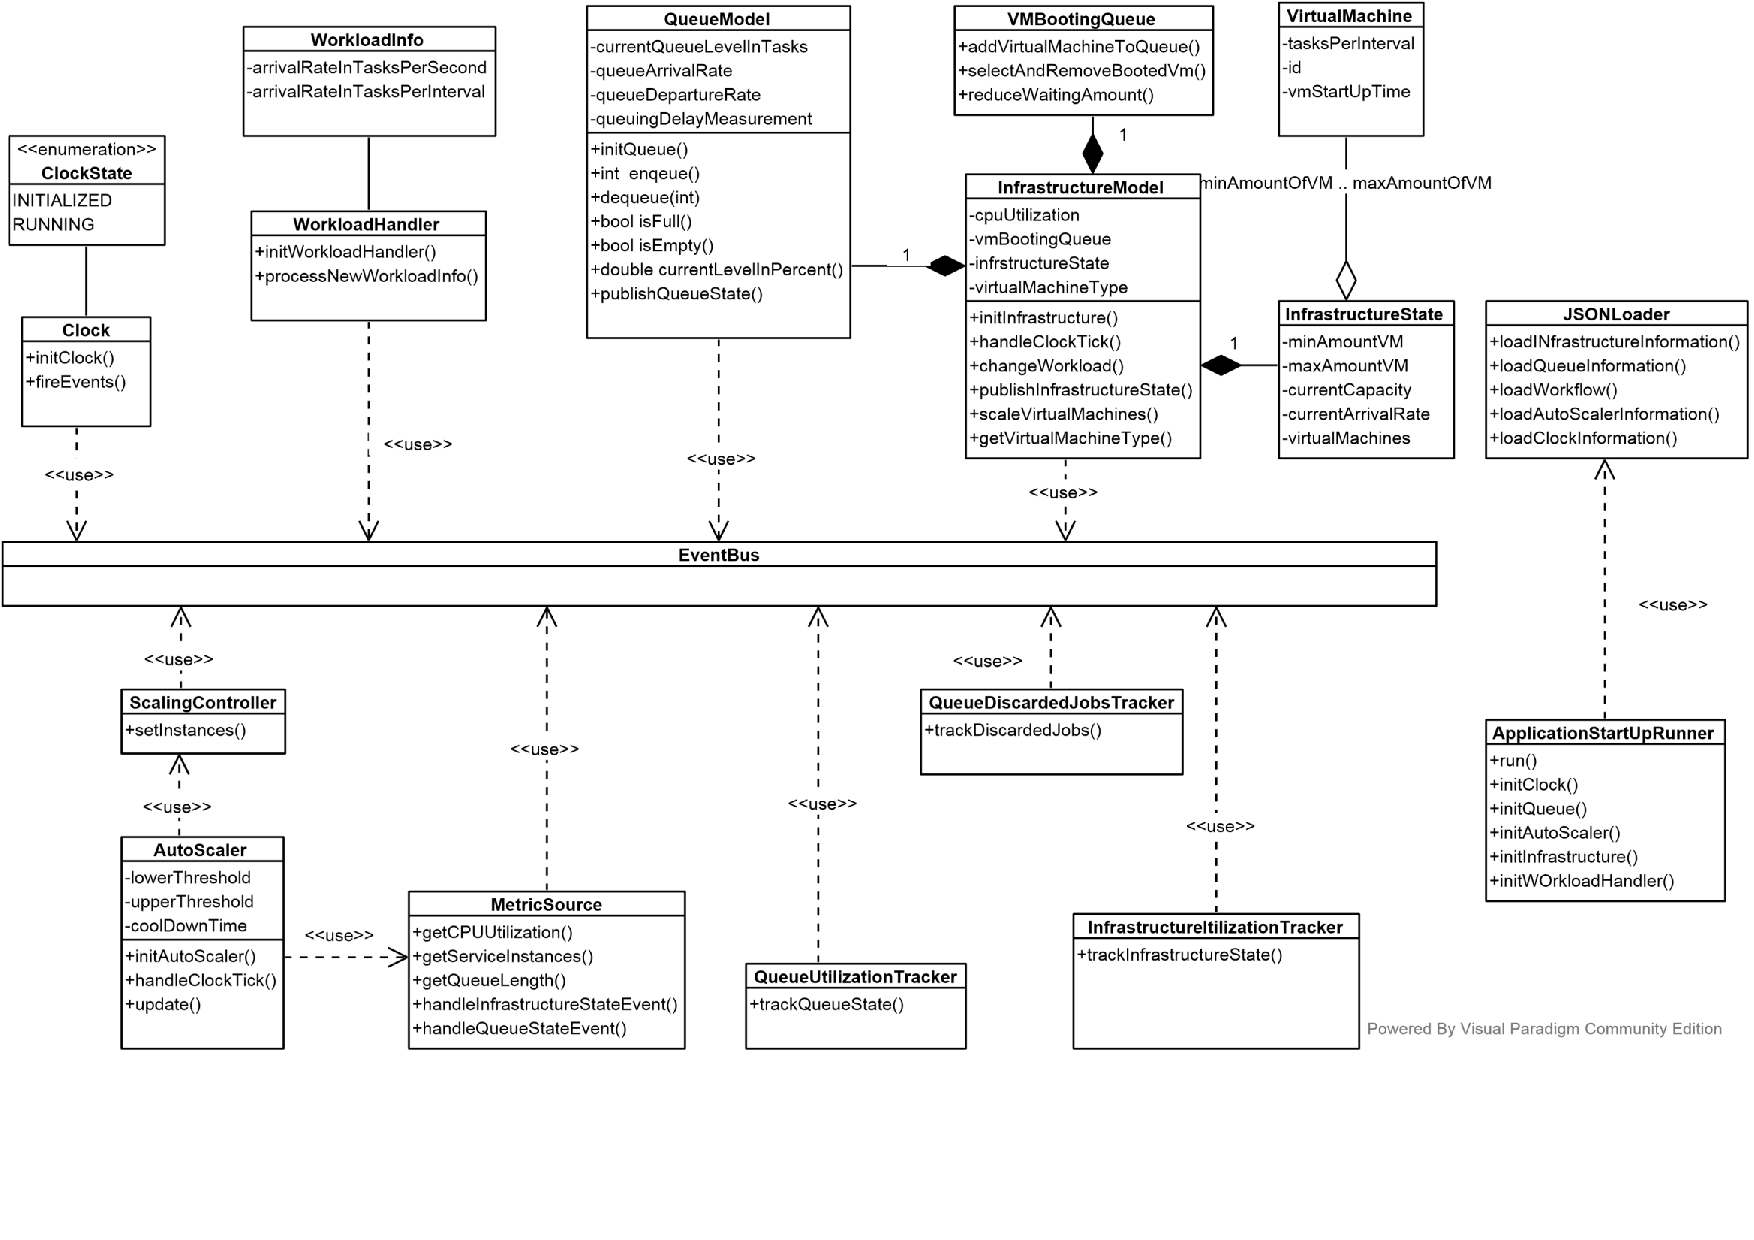
\includegraphics[width=20.0cm, trim={0cm 0cm 0cm 0cm}]{img/classDiagram.pdf}
	\end{sideways}
	\caption{Aufbau des Auto-Skalierers}
	\label{fig:classDiagram}
\end{figure}

\newpage

\subsection{Virtual Machine}
\label{sec:aufbau:VM}
Eine Virtuelle Maschine ist eindeutig durch ihre Id identifizierbar. Jede VM benötigt eine vordefinierte Zeit zum hochfahren \textit{vmStartUpTime} und kann pro Zeitintervall eine gewisse Anzahl an Jobs verarbeiten\textit{tasksPerInterval}. Die beiden letzten Werte sind bei dieser Testbench für alle Maschinen pro Simulation gleich, werden also einmalig bei Simulationsstart als Konfigurationsparameter mitgegeben.





\subsection{Auto Scaler}
Der \textit{AutoScaler} als solcher ist kein Teil der Testbench, da er ja das Testobjekt ist. In diesem Fall ist er lediglich hinzugefügt, um die Funktionalität der Testbench zu testen. Ein Auto-Scaler wird angebunden, indem er System-Metriken wie Auslastung oder Warteschlangenlänge über die Komponente \textit{MetricSource} bezieht und Skalierentscheidungen an die Komponente \textit{ScalingController} weiterreicht. Die Interfaces zur Anbindung eines Auto-Skalierers sind in Sektion\ref{sec:Konfiguration:AnbindungScaler} beschrieben.



\subsubsection{Scaling Controller}
Der \textit{ScalingController} bietet lediglich eine Schnittstelle für einen Auto-Skalierer, um Skalier-Entscheidungen an die Infrastruktur zu propagieren. Dabei wird der \textit{ScalingMode} zusammen mit den VMs, die entweder hoch- oder heruntergefahren werden sollen, übergeben.


\subsubsection{Metric Source}
Die \textit{MetricSource} bietet eine Schnittstelle für den Auto-Skalierer, um Metriken der Infrastruktur, wie bspw. die CPU-Auslastung oder die Warteschlangenlänge abzugreifen. Diese Metriken liegen immer als moving average vor, wobei das Fenster in den Konfiguration festgelegt werden kann.



\subsection{Queue Model}
\label{sec:aufbau:QueueModel}
Die Warteschlange definiert zwei grundlegende Aufgabe: Zuerst werden alle ankommenden Jobs in der Warteschlange eingereiht. Auch dann, wenn die Infrastruktur nicht völlig ausgelastet ist. Dies liegt an der Natur einer Cloud-Infrastruktur: Ein Job kann nicht in null Zeit ankommen und verarbeitet werden. Diese Verarbeitungszeit wird mit einer Warteschlange simuliert, die als FIFO-Liste aufgebaut ist. Ankommende Jobs können die Warteschlange erst verlassen, wenn sie mindestens für die Warteschlangenverzögerung \textit{(queuing delay)}. \\
Des Weiteren verhält sich die Warteschlange als Pufferspeicher: Falls die anliegende Last auf dem System größer als dessen Kapazität ist füllt sie sich. Ist es umgekehrt, so leert sie sich wieder. Da Puffer-Speicher in der Realität nicht unendlich groß sind, hat die Warteschlange eine Maximalkapazität. Ist diese erreicht, so werden weitere Jobs verworfen. \\
Wie auch das \textit{InfrastructureModel} muss die Warteschlange nach einer vordefinierten Zeit ihren Zustand publizieren, sodass \textit{Tracker} und die \textit{MetricSource} diesen auslesen können.

\subsection{Workload Handler}
Der \textit{WorkloadHandler} verarbeitet die zu simulierende Last auf dem System. Diese ist eine Eingabe als Liste von Werten. Der \textit{WorkloadHandler} verarbeitet nach einer frei konfigurierbaren Zeit den nächsten Eintrag und informiert das \textit{InfrastructureModel}, dass sie die Last geändert hat. Damit wird umgangen, dass tatsächlich Last generiert werden muss. Die Infrastruktur bekommt lediglich Informationen darüber, zu welchem Zeitpunkt wie viel Last anliegt. 

\subsubsection{Workload Info}
\textit{WorkloadInfo} ist eine Klasse, die eine Last zu einem bestimmten Zeitpunkt beschreibt.

\subsection{Tracker}
Die verschiedenen \textit{Tracker} zeichnen die Simulation zeit-diskret auf. Die Informationen können anschließend benutzt werden, um den Auto-Skalierer zu beurteilen. Alle aufgezeichneten Parameter werden durch Aufzeichnung der Zustände der jeweiligen Komponenten erhoben. Dabei wird ein gleitender Mittelwert bestimmt, um glattere Ergebnisse zu bekommen.

\subsubsection{Queue Utilization Tracker}
Dieser \textit{Tracker} zeichnet folgende Parameter auf:
\begin{itemize}
	\item Anzahl an wartenden Jobs 
	\item Füllstand in Prozent, gemessen an der maximalen Länge
	\item Ankunftsrate
	\item Verarbeitungsrate (Menge an Jobs, die die  Warteschlange verlassen)
	\item Durchschnittliche Wartezeit in der Warteschlange
\end{itemize}

\subsubsection{Queue Discarded Jobs Tracker}
Dieser \textit{Tracker} zeichnet folgende Parameter auf:
\begin{itemize}
	\item Anzahl an verworfenen Jobs Pro Intervall
\end{itemize}

\subsubsection{Infrastructure Utilization Tracker}
\begin{itemize}
	\item Ankunftsrate
	\item Verarbeitungsrate (Menge an Jobs, die das System verlassen)
	\item Kapazität (Menge an Jobs, die alle VMs verarbeiten können)
	\item Anzahl der Virtuellen Maschinen
	\item CPU Auslastung
\end{itemize}

\subsection{Application Start Up Runner}
Diese Komponente liest die Konfigurationen via \textit{JSONLoader} und initialisiert alle anderen Komponenten. Dies beinhaltet die Umrechnung der externen Einheit (Parameter gegeben in Millisekunden) in die interne Einheit (gegeben in Clock-Ticks). Anschließend startet sie die Simulation.

\subsection{JSON Loader}
Der \textit{JSONLoader} ist eine Klasse zum laden und serialisieren der Konfigurationen im JSON-Format. Jede Konfigurations-Datei wird dabei mittels \textit{Object-Mapper} auf eine Klasse abgebildet.

\section{Events}
\label{sec:Aufbau:Events}
Für die Kommunikation zwischen den Komponenten, beziehungsweise um das Auslösen einer Handlung (Methodenaufruf) einer speziellen Komponente anzustoßen, werden Events benutzt. Abbildung \ref{fig:eventsDiagram} zeigt, dass alle Events von einem \textit{AbstractEvent} erben, in dem der aktuelle Clock-Zähler und die feste Intervall-Dauer gegeben ist. Diese Informationen sind somit in jedem Event verfügbar, sodass man das Event einem diskreten Zeitintervall zuordnen kann. Im folgenden wird darauf eingegangen, was ein Event absetzt und für was es bestimmt ist.\\
In dieser Applikation wird mit synchronen Events gearbeitet, das heißt, dass nach Erhalt eines Events durch einen Listener zuerst der gesamte Code auszuführen ist, bevor es an der Stelle weitergeht, an der das Event geworfen wurde. Falls mehr als ein Listener auf ein geworfenes Event reagiert, wird der Code aller Listener-Methoden nacheinander abgearbeitet. Jedoch ist nicht spezifiziert, in welcher Reihenfolge das geschieht, da dies vom Spring-Framework verwaltet wird. Falls also eine Ordnung der Ausführung erzwungen werden soll, müssen zwei verschiedene Event-Typen definiert werden. Diese können dann in der gewünschte Reihenfolge auf den Event-Bus gelegt werden. Die synchrone Abarbeitung garantiert, dass der Code des Listeners, der auf das erste Event hört zuerst vollständig bearbeitet wird.



\begin{itemize}


	\item \textit{FinishSimulationEvent} 
	\begin{itemize}
         \item \textbf{Absender:} \textit{Clock}
         \item \textbf{Empfänger:} Alle Tracker
         \item \textbf{Grund:} Erstellen der Ausgabedateien, Schließen der File-Writer
         \item \textbf{Parameter:} Skalierfaktor, zurückrechnen in Ausgabeformat
 	\end{itemize} 
     
    	\item \textit{StartSimulationEvent} 
    \begin{itemize}
    	\item \textbf{Absender:} \textit{Clock}
    	\item \textbf{Empfänger:} Alle Tracker
    	\item \textbf{Grund:} Beenden des Schreibens in die jeweiligen Dateien
    \end{itemize} 

\pagebreak

	\item \textit{ClockEvent} 
\begin{itemize}
	\item \textbf{Absender:} \textit{Clock}
	\item \textbf{Empfänger:} \textit{InfrastructureModel}, \textit{AutoScaler}
	\item \textbf{Grund:} Beginn neues Intervall
\end{itemize} 

	\item \textit{TriggerPublishInfrastructureStateEvent} 
\begin{itemize}
	\item \textbf{Absender:} \textit{Clock}
	\item \textbf{Empfänger:}  \textit{InfrastructureModel}
	\item \textbf{Grund:} Infrastruktur soll Zustand publizieren
\end{itemize} 

	\item \textit{TriggerPublishQueueStateEvent} 
\begin{itemize}
	\item \textbf{Absender:} \textit{Clock}
	\item \textbf{Empfänger:} \textit{QueueModel}
	\item \textbf{Grund:} Warteschlange soll Zustand publizieren
\end{itemize} 

	\item \textit{TriggerWorkloadHandlerEvent} 
\begin{itemize}
	\item \textbf{Absender:} \textit{Clock}
	\item \textbf{Empfänger:} \textit{WorkloadHandler}
	\item \textbf{Grund:} Neue Workload publizieren
\end{itemize} 

	\item \textit{ScalingEvent} 
\begin{itemize}
	\item \textbf{Absender:} \textit{ScalingController}
	\item \textbf{Empfänger:} \textit{InfrastructureModel}
	\item \textbf{Grund:} Neue Skalier-Entscheidung getroffen
	\item \textbf{Parameter:} Skalier-Modus und jeweilige VM-Instanzen
\end{itemize} 

	\item \textit{QueueStateEvent} 
\begin{itemize}
	\item \textbf{Absender:} \textit{QueueModel}
	\item \textbf{Empfänger:} \textit{QueueTracker}
	\item \textbf{Grund:} Zustand der Warteschlange soll geschrieben werden
	\item \textbf{Parameter:} Enthält Infos über Zustand, die in Datei geschrieben werden sollen
\end{itemize} 



	\item \textit{WorkloadChangedEvent} 
\begin{itemize}
	\item \textbf{Absender:} \textit{WorkloadHandler}
	\item \textbf{Empfänger:} \textit{InfrastructureModel}
	\item \textbf{Grund:} Veränderung der Workload
	\item \textbf{Parameter:} Neue Workload
\end{itemize} 



\pagebreak




	\item \textit{DiscardedJobsEvent} 
\begin{itemize}
	\item \textbf{Absender:} \textit{QueueModel}
	\item \textbf{Empfänger:} \textit{QueueTracker}
	\item \textbf{Grund:} Jobs wurden verworfen, da Warteschlange übergelaufen ist
	\item \textbf{Parameter:} Anzahl der verworfenen Jobs im Zeitintervall
\end{itemize} 

	\item \textit{InfrastructureStateEvent} 
\begin{itemize}
	\item \textbf{Absender:} \textit{InfrastructureModel}
	\item \textbf{Empfänger:} \textit{InfrastructureTracker}
	\item \textbf{Grund:}  Zustand der Infrastruktur soll geschrieben werden
	\item \textbf{Parameter:} Enthält Infos über Zustand, die in Datei geschrieben werden sollen
\end{itemize} 





\end{itemize}
 

%"l, b, r, t"
\begin{figure}[!h]
	\centering
	
	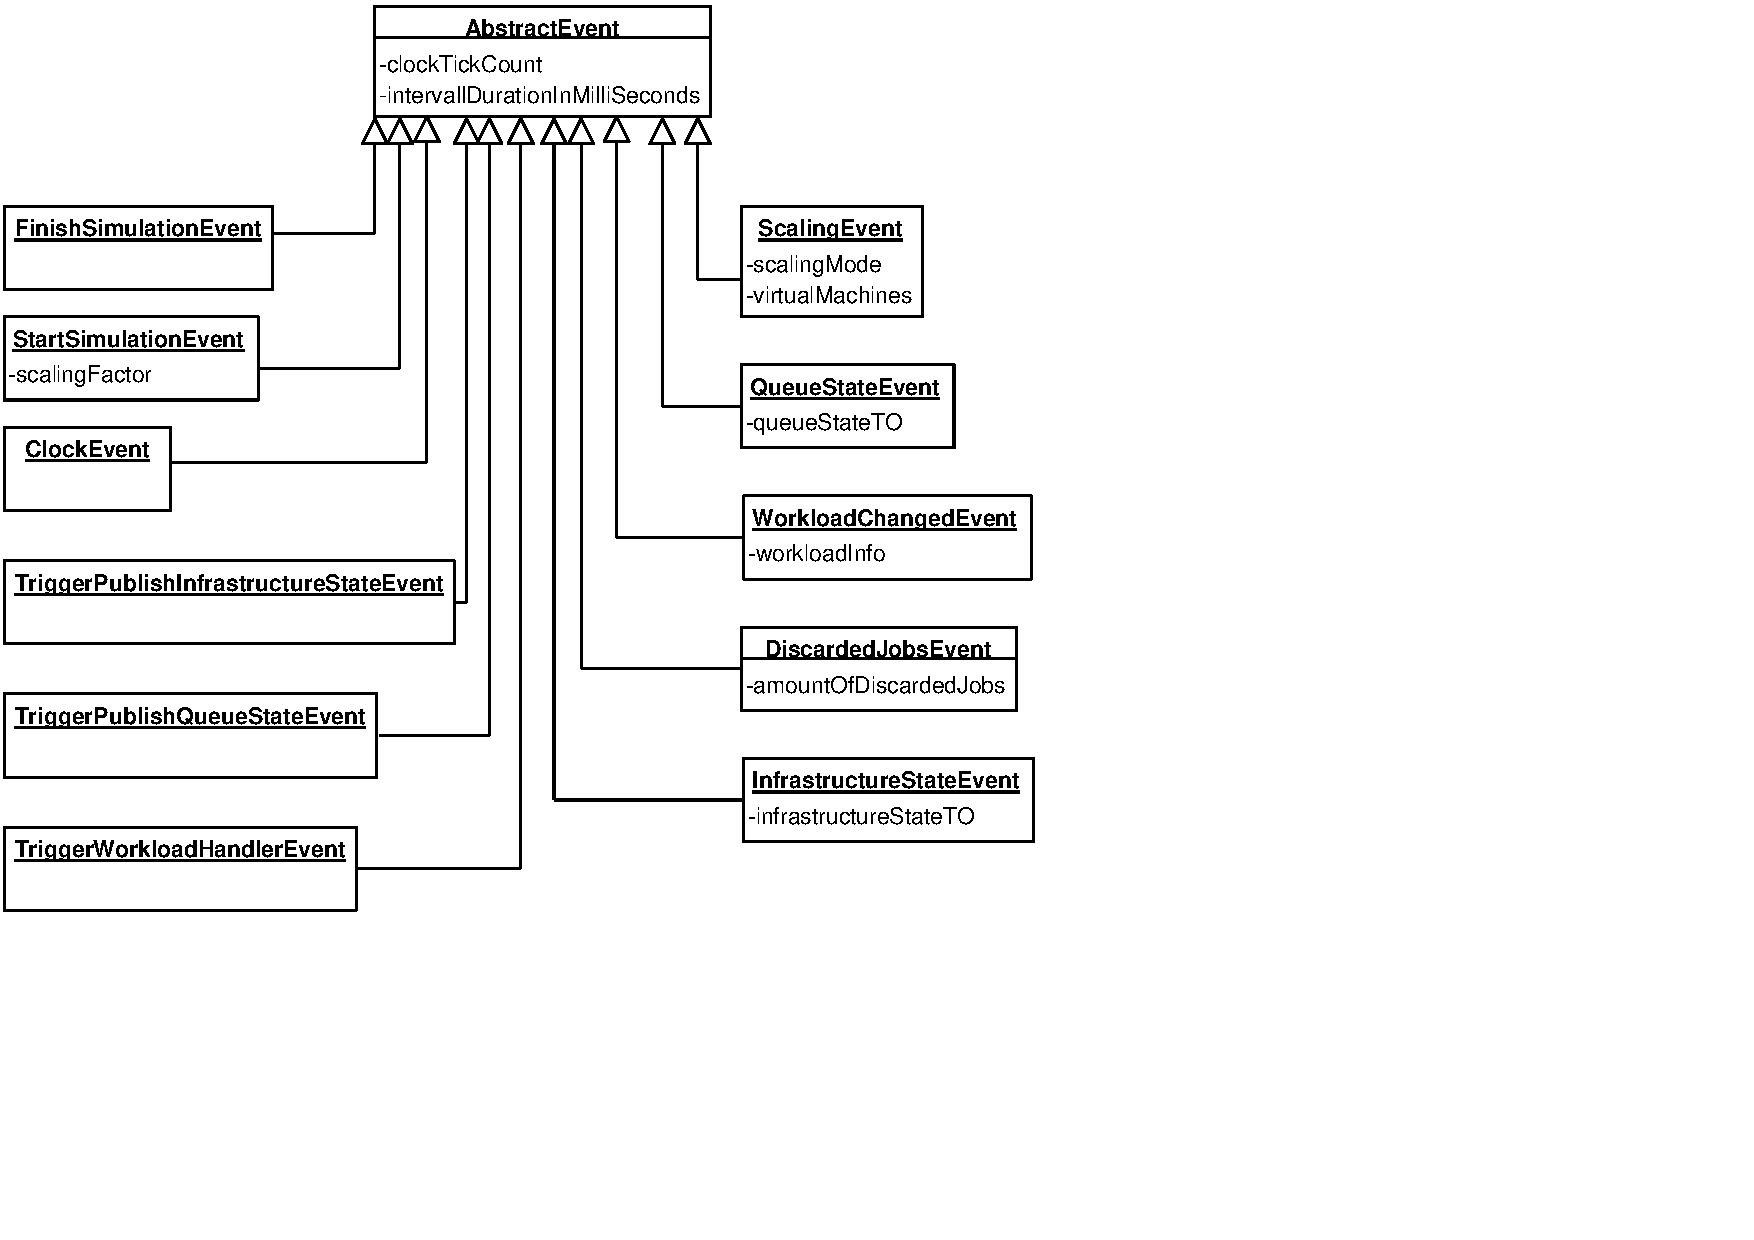
\includegraphics[width=20.0cm, trim={0cm 5cm 6cm 0cm}]{img/eventsDiagram.pdf}
	
	\caption{Übersicht der Events}
	\label{fig:eventsDiagram}
\end{figure}




\section{Ablauf}
Das Sequenzdiagramm in Abbildung \ref{fig:ablauf} verdeutlicht den Ablauf eines Simulationszyklus. Wie in Sektion \ref{sec:Aufbau:Events} beschrieben, werden die Event synchron empfangen. Falls in der Abbildung ausgehend von einer Komponente zwei mal das Selbe Event direkt hintereinander gesendet wird (bspw. \textit{startSimulation()}), so ist dessen Ausführungsreihenfolge nicht definiert. In der Applikation wird dieses Event nur ein mal auf den Event-Bus gelegt, allerdings von zwei Listener entnommen. \\
Nachdem die Konfigurationen gelesen und die Komponenten initialisiert wurden, wird die \textit{Clock} gestartet. Zuerst werden die \textit{Tracker} initialisiert, da diese je einen \textit{File-Writer} erstellen, mit denen später die Zustandsinformationen geschrieben werden können. Daraufhin startet die eigentliche Simulation. Die Schleife wird sooft durchlaufen, bis die vorkonfigurierte Simulationszeit verstrichen ist. \\
Im gesamten Sequenzdiagramm befinden sich mehrere Ausführungen, die nur unter gewissen Bedingung ausgeführt werden. Im folgenden wird der Zyklus ein mal komplett durchlaufen, mit der Prämisse, dass alle Bedingungen erfüllt wären. \\
Der \textit{WorkloadHandler} wird periodisch, nach einer vorgegebenen Anzahl Zyklen angestoßen. Der neue Workload wird geladen und an das \textit{InfrastructureModel} weitergegeben. Dort wird die alte Workload mit der neuen ersetzt, was bedeutet, dass entweder mehr oder weniger Jobs pro Zeitintervall ankommen (bis sich die Workload wieder ändert). \\
Auch der \textit{AutoScaler} wird periodisch, nach einer vorgegebenen Anzahl Zyklen angestoßen. Falls er nicht in der CoolDown-Phase ist (Zeit nach einer vergangenen Skalier-Entscheidung, in der er nichts machen soll), holt er sich die benötigten Metriken von der \textit{MetricSource}, wie bspw. CPU-Auslastung. Skalier-Entscheidungen werden dann an die Schnittstelle (\textit{ScalingController}) gegeben, die die Informationen über den Event-Bus an das \textit{InfrastructureModel} sendet. Dort angekommen wird die Skalier-Entscheidung ausgeführt. Im Falle einer Hinzunahme weiterer VMs, werden diese in die \textit{VMBootingQueue} eingereiht. Das Abschalten einer VM funktioniert ohne weiteres Warten. \\
Sobald das \textit{InfrastructureModel} angestoßen wird, wird überprüft ob neue VMs hochgefahren sind. Ist dies der Fall, so werden diese zur Infrastruktur hinzugefügt und damit die Kapazität erhöht. Anschließend werden, basierend auf der aktuellen Workload, eine Anzahl an Jobs in die Warteschlange eingereiht. Danach werden, basierend auf der gegenwärtigen Kapazität, eine Anzahl an Jobs der Warteschlange entnommen. Sowohl bei dem \textit{QueueModel} als auch bei dem \textit{InfrastructureModel} werden dabei diverse Metriken erhoben und als gleitender Mittelwert gespeichert. Zuletzt wird die Wartezeit noch nicht hochgefahrener VMs dekrementiert, sodass diese ggf. im nächsten Iterationsschritt hinzugefügt werden können. \\
Im letzten Schritt einer Iterationszyklus, werden \textit{InfrastructureModel} und \textit{QueueModel} aufgefordert, ihren Zustand zu verbreiten. Die Informationen gehen im ersten Fall an den \textit{InfrastructureTracker} und im zweiten Fall an den \textit{QueueTracker}. Beides wird ebenfalls von der \textit{MetricSource} benutzt, um für diverse Metriken, die aus den Zustandsinformationen erhoben werden können, je einen gleitenden Mittelwert zu bilden. \\
Dieser Zyklus wiederholt sich, bis die Anzahl der durchlaufenen Zyklen der Simulationszeit entspricht. Zuletzt werden noch die \textit{File-Writer} in den \textit{Tracker} geschlossen und die Simulation ist beendet.  

 

%"l, b, r, t"
\begin{figure}[!h]
	\centering
	\begin{sideways}
	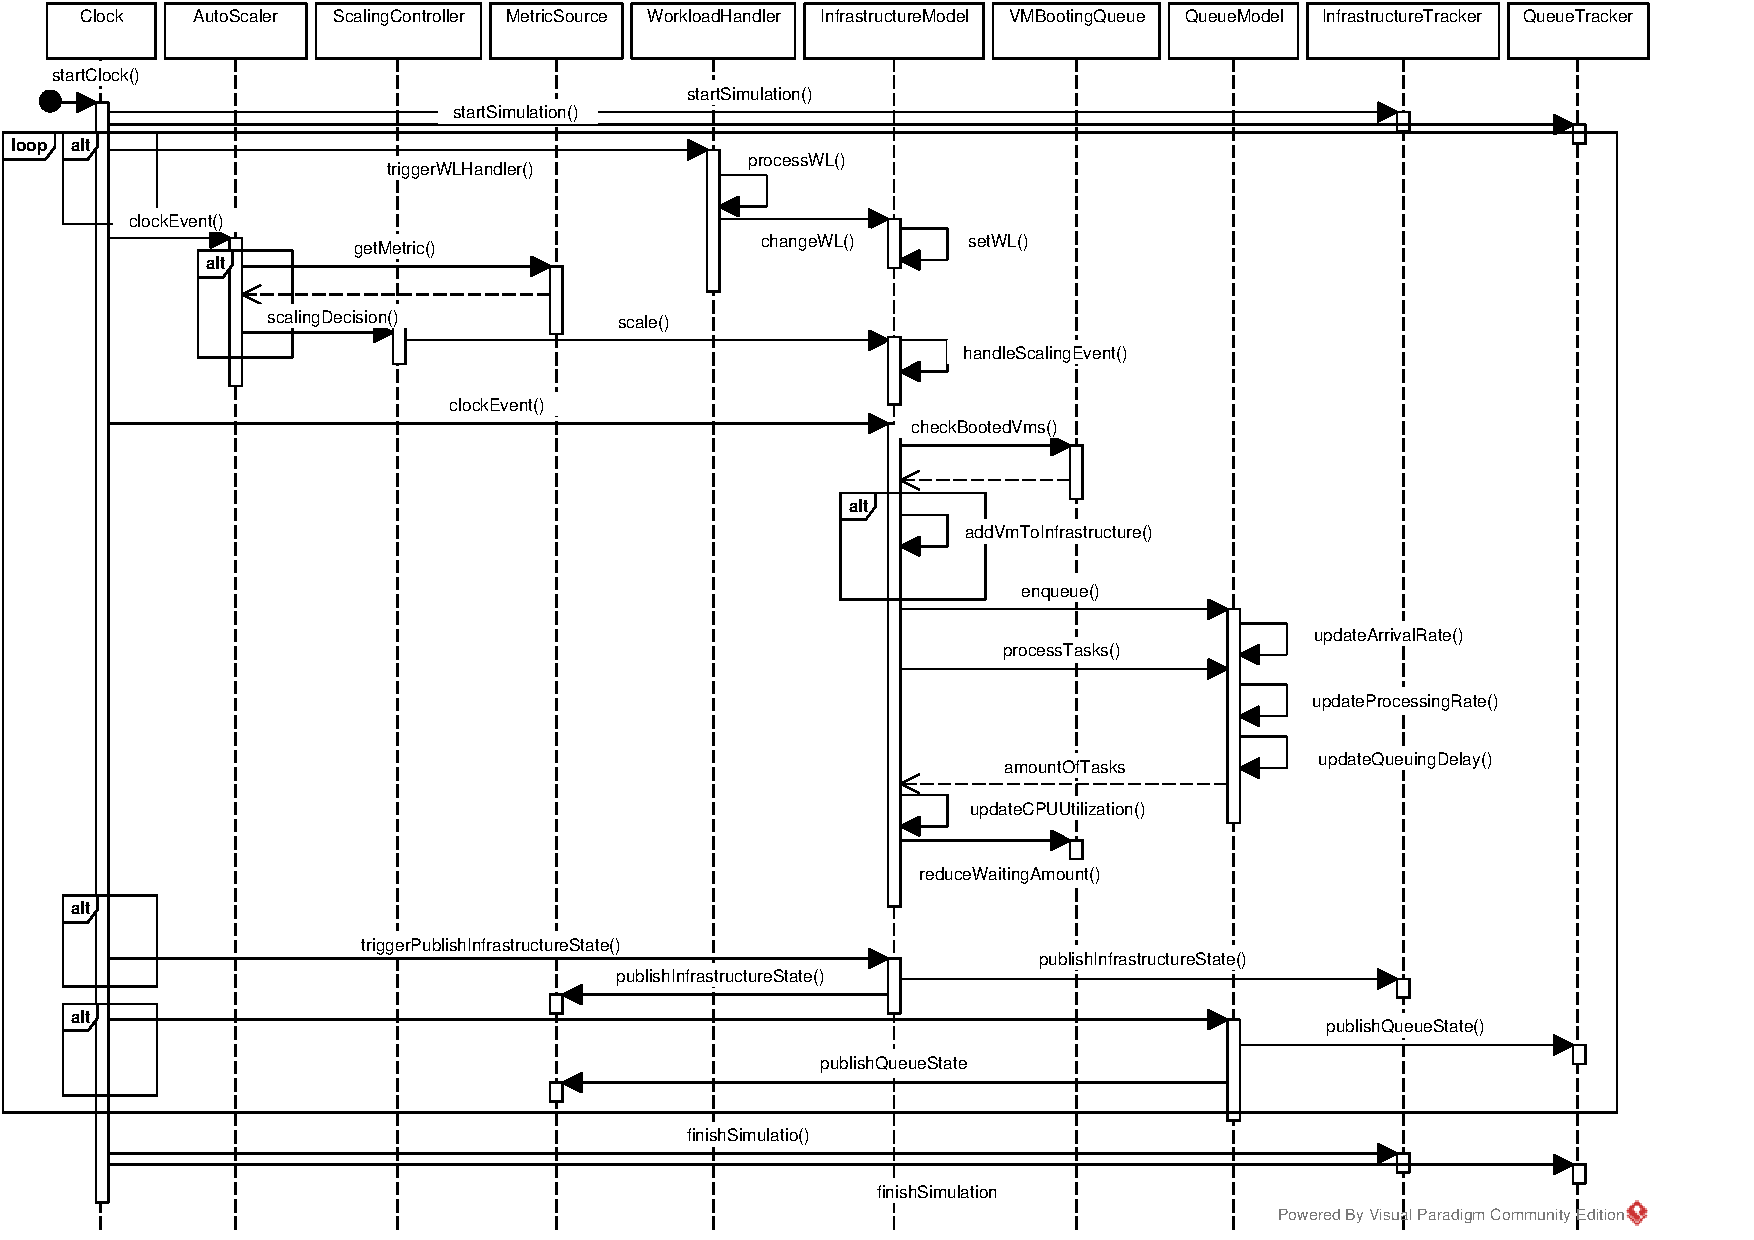
\includegraphics[width=22cm, trim={0cm 0cm 2cm 1cm}]{img/ablauf.pdf}
	\end{sideways}
	\caption{Ablauf der zeit-diskreten Simulation}
	\label{fig:ablauf}
\end{figure}



